
\documentclass{article}
\usepackage[headheight=20pt, margin=1.0in, top=1.2in]{geometry}
\usepackage{amsmath, amssymb, amsthm, thmtools, tcolorbox, array, graphicx, makeidx, cancel, multirow, fancyhdr, xypic, color, nicefrac, rotating, multicol, caption, subcaption, xcolor, tikz, tikz-3dplot, tikz-cd, pgfplots, import, enumitem, calc, booktabs, wrapfig, siunitx, hyperref,float}
\hypersetup{colorlinks=true,linkcolor=blue}
\usepackage[all]{xy}
\usepackage{esint}
\setlength{\parindent}{0in}
\sisetup{per-mode = symbol}
\usetikzlibrary{calc,arrows,svg.path,decorations.markings,patterns,matrix,3d,fit}
\usepgfplotslibrary{groupplots}
\pgfplotsset{compat=newest}
\newtcolorbox{mydefbox}[2][]{colback=red!5!white,colframe=red!75!black,fonttitle=\bfseries,title=#2,#1}
\newtcolorbox{mythmbox}[2][]{colback=gray!5!white,colframe=gray!75!black,fonttitle=\bfseries,title=#2,#1}
\newtcolorbox{myexamplebox}[2][]{colback=green!5!white,colframe=green!75!black,fonttitle=\bfseries,title=#2,#1}
\newtcolorbox{mypropbox}[2][]{colback=blue!5!white,colframe=blue!75!black,fonttitle=\bfseries,title=#2,#1}
\declaretheoremstyle[headfont=\color{blue}\normalfont\bfseries,]{colored}
\theoremstyle{definition}
\newtheorem{theorem}{Theorem}
\newtheorem{corollary}[theorem]{Corollary}
\newtheorem{lemma}[theorem]{Lemma}
\newtheorem{proposition}[theorem]{Proposition}
\newtheorem{problem}[theorem]{Problem}
\newtheorem{definition}[theorem]{Definition}
\newtheorem{exercise}[theorem]{Exercise}
\newtheorem{example}[theorem]{Example}
\newtheorem{solution}[theorem]{Solution}
\newtheorem*{thm}{Theorem}
\newtheorem*{lem}{Lemma}
\newtheorem*{prob}{Problem}
\newtheorem*{exer}{Exercise}
\newtheorem*{prop}{Proposition}
\def\R{\mathbb{R}}
\def\F{\mathbb{F}}
\def\Q{\mathbb{Q}}
\def\C{\mathbb{C}}
\def\N{\mathbb{N}}
\def\Z{\mathbb{Z}}
\def\Ra{\Rightarrow}
\def\e{\epsilon}
\newcommand{\typo}[1]{{\color{red}{#1}}}
\newcommand\thedate{\today}
\newcommand{\mb}{\textbf}
\newcommand{\norm}[2]{\|{#1}\|_{#2}}
\newcommand{\normm}[1]{\|#1\|}
\newcommand{\mat}[1]{\begin{bmatrix} #1 \end{bmatrix}}
\newcommand{\eqtext}[1]{\hspace{3mm} \text{#1} \hspace{3mm}}
\newcommand{\set}[1]{\{#1\}}
\newcommand{\inte}{\textrm{int}}
\newcommand{\ra}{\rightarrow}
\newcommand{\minv}{^{-1}}
\newcommand{\tx}[1]{\text{ {#1} }}
\newcommand{\abs}[1]{|#1|}
\newcommand{\mc}[1]{\mathcal{#1}}
\newcommand{\uniflim}{\mathop{\mathrm{unif\lim}}}
\newcommand{\notimplies}{\mathrel{{\ooalign{\hidewidth$\not\phantom{=}$\hidewidth\cr$\implies$}}}}
\pagestyle{fancy}
\fancyhf{}
\fancyhead[L]{Title of the Document}
\fancyhead[C]{}
\fancyhead[R]{\thepage}
\fancyfoot[L]{}
\fancyfoot[C]{}
\fancyfoot[R]{}
\renewcommand{\headrulewidth}{0.4pt}
\renewcommand{\footrulewidth}{0.4pt}
\numberwithin{equation}{section}
% Increase spacing between paragraphs
\setlength{\parskip}{1em}
% Increase spacing before and after sections
\usepackage{titlesec}
\titlespacing*{\section}{0pt}{3ex plus 1ex minus .2ex}{2ex plus .2ex}
\titlespacing*{\subsection}{0pt}{2ex plus 1ex minus .2ex}{1ex plus .2ex}
\titlespacing*{\subsubsection}{0pt}{1ex plus 1ex minus .2ex}{1ex plus .2ex}
\title{\textbf{Title of the Document}}
\author{Author Name}
\date{\today}
\begin{document}
\maketitle
\tableofcontents
\newpage
\section{Exercises}
\begin{enumerate}
    \item Let $(X,d)$ be a metric space and $S \subseteq X$. Show that $\partial S = \partial S^c$.
    \item Show that for an arbitrary choice of \(a, b, r \in \mathbb{R}\), the closed disk \((x - a)^2 + (y - b)^2 \le r^2\) is a bounded set in \(\mathbb{R}^2\).
    \item Let $f:(X,d) \to (Y,d)$ be a metric space and for \(x,y \in X\). Show that if $d(f(x), f(y)) < \epsilon$ for every \(\epsilon > 0\), then \( x = y\).
\end{enumerate}

\subsection*{Exercise 1}
Assume $\partial S \neq \partial S^c$. $\exists x \in \partial S, x \notin \partial S^c$. Then by \(x \in \partial S \Rightarrow \forall \epsilon > 0: B_\epsilon(x) \cap S \neq \emptyset \). However, by \(x \notin \partial S^c\), this value of \(\epsilon > 0\) implies \(B_\epsilon(x) \cap S = \emptyset \Rightarrow B_\epsilon(x) \subseteq S^c\), which is a contradiction, implying our assumption that $x \in \partial S \setminus \partial S^c$ must be false and $\partial S \cap \partial S^c = \emptyset$.

\subsection*{Exercise 2}
A set \(S\) is bounded iff \(\exists M \in \mathbb{R}^+ \, \forall x,y \in S \, d(x,y) < M\).

Let \(a, b, r \in \mathbb{R}\). 

$
S := \{(x,y) \in \mathbb{R}^2 \mid (x-a)^2 + (y-b)^2 \leq r^2\}
$

$
\Rightarrow x^2 - 2ax + a^2 + y^2 - 2yb + b^2 \le r^2 
$

$
\Rightarrow x^2 - 2ax + y^2 - 2yb \le r^2 - a^2 - b^2
$

$
\Rightarrow x^2 + y^2 \le r^2 - a^2 - b^2 + 2ax + 2yb
$

We need to show \(x^2\) is bounded:
$
(x - a)^2 \le r^2
$

$
\Rightarrow |x - a| \le |r|
$

$
\Rightarrow |x - a| \le |r| \implies |x - a| \le |r| + |a| 
$

$
\Rightarrow |x| = |x - a + a| \le |x - a| + |a| \le r + |a|
$

$
\Rightarrow |x| \le r + |a|
$

Thus, \(x\) is bounded, and similarly we can show for \(y\). Therefore, \(S\) is bounded.

\begin{align*}
& \text{Consider the circle:} \\
& 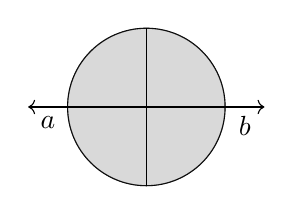
\begin{tikzpicture}
\draw (0,0) circle (1);
\draw[fill=gray,opacity=0.3] (0,0) circle (1);
\draw (-1,0) -- (1,0);
\draw (0,-1) -- (0,1);
\draw[<-] (-1.5,0) -- (-1,0) node[midway,below] {\( a \)};
\draw[->] (1,0) -- (1.5,0) node[midway,below] {\( b \)};
\end{tikzpicture} \\
& \Rightarrow |y| \leq r + |a| \\
& \Rightarrow y^2 \leq (r + |a|)^2 \\
& \text{Same for } y, \quad y^2 \leq (r + |b|)^2 \\
& \forall z = (x, y) \in \mathbb{D}_{x,y}^2, \\
& \quad \|z\| = \sqrt{x^2 + y^2} \\
&\leq \sqrt{(r + |a|)^2 + (r + |b|)^2}
\end{align*}

Thus, if \( M = \sqrt{(r + |a|)^2 + (r + |b|)^2} \), the bound holds.

\#1S named boundness = distance boundness.

\begin{align*}
\text{Let } & x = (x_1, x_2), \quad y = (y_1, y_2) \in \mathbb{R}^2, \\
& z = \{x, y\} \\
& (x_2 - a)^2 + (y_2 - b)^2 = r^2 \\
\Rightarrow & d(z, (a, b)) = \sqrt{(x_2 - a)^2 + (y_2 - b)^2} \leq r \\
\Rightarrow & d(x, y) \leq d(x, (a, b)) + d((a, b), y) \\
& = \sqrt{(x_1 - a)^2 + (x_2 - b)^2} + \sqrt{(y_1 - a)^2 + (y_2 - b)^2} \\
& \leq r + r = 2r.
\end{align*}

\noindent
\textbf{(iii) Suppose that \( x \neq y \). Then \( d(x,y) \neq 0 \). Thus if we choose \( \epsilon = d(x,y) \Rightarrow \epsilon > 0 \) but \( d(x,y) \not \in \epsilon \). (contradiction).}

\noindent
\textbf{(contradiction) Suppose \( x = y \) and so \( d(x,y) \neq 0 \).}

$
\text{choose } \epsilon > 0 \text{ so that } \epsilon = d(x,y). \quad \text{Then we must have} \quad d(x,y) < \epsilon = d \left( \frac{\epsilon}{2} \right)  =  \frac{\epsilon}{2} \quad \text{, which is a contradiction, as this implies} 
$
$
\text{if } d(x,y) \leq 0 \Rightarrow d(x,y) = \epsilon < \epsilon = \frac{\epsilon}{2} 
$
$
 \Rightarrow s \leq \frac{\epsilon}{2} \Rightarrow \frac{3\epsilon}{2} \leq \frac{\epsilon}{2} 
$
$
 \text{Thus} \quad x = y. 
$

\newpage

\noindent
\textbf{(iv) Let \((V, \|\cdot\|)\) be a normed vsp. }

\noindent
\textbf{Then let \(r > 0\) and \(x \in V\). Then}
$
B_r(x) = \left \{u \in V | d(x,u) < r \right \}
 $
$
 B_{r+ \|x\|}(0) = \left \{v \in V | d(0,v) < r + \|x\| \right \}
 $

$
\text{Let } y \in B_r(x).\\
$
$
d(0,y) \leq d(0,x) + d(x,y) \\
 $
$
\leq \|x\| + r.
 $
 $
 \Rightarrow B_r(x) \subseteq B_{r + \|x\|}(0).
 $

\newpage

\noindent
\textbf{(v) Suppose \(S\) is bounded. Then \(\exists M \in \mathbb{R} : \forall x \in S \|x\| \leq M.
\)

$
\text{(Equiv to } \exists M \in \mathbb{R} : \forall x \in S x \in B_M(0))
 $\end{document}